\documentclass[tikz,border=12pt]{standalone}
\usepackage{graphicx}
\usepackage{amsmath,amssymb}
\usepackage{tikz}
\usetikzlibrary{arrows.meta,positioning,fit,calc,backgrounds}
\tikzset{
  box/.style={
    draw,
    very thick,
    rectangle,
    align=center,
    inner sep=8pt,
    minimum height=1.25cm,
    minimum width=3.1cm,
    font=\small,
  },
  wide/.style={box, minimum width=3.6cm},
  arr/.style={-{Stealth[length=2.6mm, width=2mm]}, thick},
  barr/.style={
    {Stealth[length=2.4mm, width=1.8mm]}-{Stealth[length=2.4mm, width=1.8mm]},
    thick,
  },
  lbl/.style={font=\scriptsize, inner sep=2pt, fill=white},
  group/.style={draw, dashed, inner sep=12pt},
}

\begin{document}
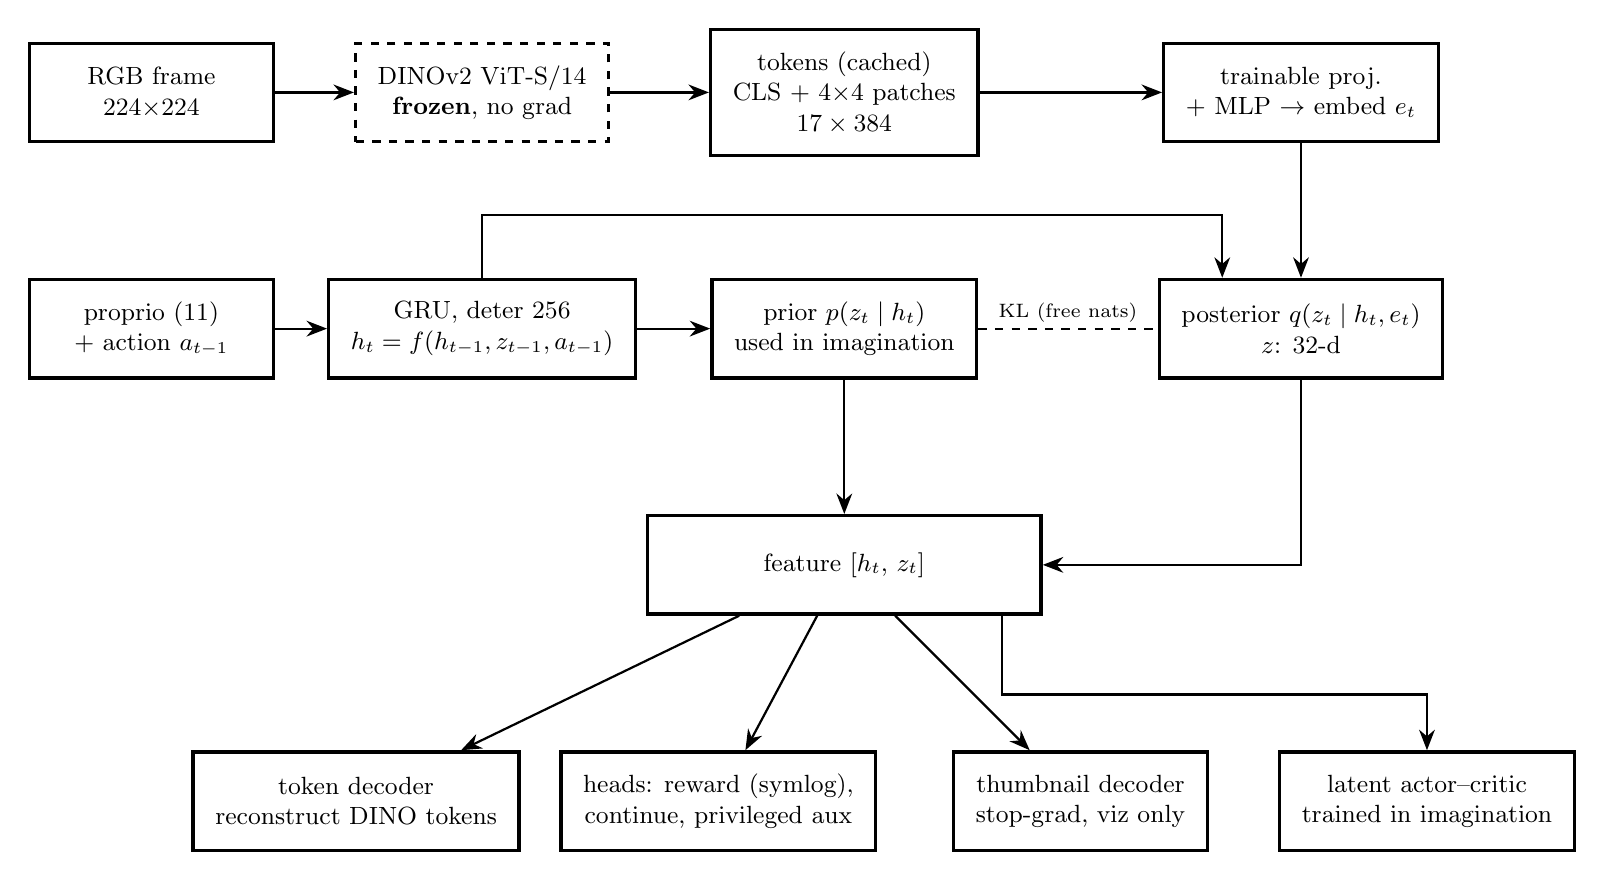
\begin{tikzpicture}
  % row 1: perception (frozen)
  \node[box] (frame) at (0,0) {RGB frame\\$224{\times}224$};
  \node[box, dashed] (dino) at (4.2,0) {DINOv2 ViT-S/14\\\textbf{frozen}, no grad};
  \node[box] (tok) at (8.8,0) {tokens (cached)\\CLS $+$ $4{\times}4$ patches\\$17\times384$};
  \node[box] (proj) at (14.6,0) {trainable proj.\\+ MLP $\to$ embed $e_t$};
  \draw[arr] (frame) -- (dino);
  \draw[arr] (dino) -- (tok);
  \draw[arr] (tok) -- (proj);

  % row 2: RSSM
  \node[box] (gru) at (4.2,-3) {GRU, deter 256\\$h_t=f(h_{t-1},z_{t-1},a_{t-1})$};
  \node[box] (prior) at (8.8,-3) {prior $p(z_t\mid h_t)$\\used in imagination};
  \node[box] (post) at (14.6,-3) {posterior $q(z_t\mid h_t,e_t)$\\$z$: 32-d};
  \node[box] (prop) at (0,-3) {proprio (11)\\$+$ action $a_{t-1}$};
  \draw[arr] (prop) -- (gru);
  \draw[arr] (gru) -- (prior);
  \draw[arr] (proj) -- (post);
  \draw[arr] (gru.north) -- ++(0,0.8) -| ([xshift=-1cm]post.north);
  \draw[dashed, thick] (prior.east) -- node[lbl, above] {KL (free nats)} (post.west);

  % row 3: feature
  \node[box, minimum width=5cm] (feat) at (8.8,-6) {feature $[h_t,\,z_t]$};
  \draw[arr] (prior.south) -- (feat.north);
  \draw[arr] (post.south) |- (feat.east);

  % row 4: heads
  \node[box] (dec) at (2.6,-9) {token decoder\\reconstruct DINO tokens};
  \node[box] (hd) at (7.2,-9) {heads: reward (symlog),\\continue, privileged aux};
  \node[box] (thumb) at (11.8,-9) {thumbnail decoder\\stop-grad, viz only};
  \node[box] (ac) at (16.2,-9) {latent actor--critic\\trained in imagination};
  \draw[arr] (feat) -- (dec);
  \draw[arr] (feat) -- (hd);
  \draw[arr] (feat) -- (thumb);
  \draw[arr] (feat.south) ++(2,0) -- ++(0,-1.0) -| (ac.north);
\end{tikzpicture}
\end{document}
